\documentclass[11pt]{article}

\usepackage[hmargin=1in,vmargin=0.8in]{geometry}
\usepackage{listings}
\usepackage{color}
\usepackage{hyperref}
\usepackage{graphicx}

% For better handling of unicode (Latin characters, anyway)
\IfFileExists{lmodern.sty}{\usepackage{lmodern}}{}
\usepackage[T1]{fontenc}
\usepackage[utf8]{inputenc}

\hypersetup{
    colorlinks=true,
    linkcolor=blue,
    urlcolor=red,
    linktoc=all
}

% bibliographie
\RequirePackage{filecontents}
\begin{filecontents*}{bibliografie.bib}
	@misc{sourceCode,
		author = "PEREIRA Romain",
		title = "Source code",
		howpublished = "\newline\url{https://github.com/rpereira-dev/VoxelEngine.git}",
		note = "\newline The main repository of the project"
	}
\end{filecontents*}

% title setup
\title{Title goes here}
\author{Author goes there}
\date{30th October 2017}

\renewcommand*\contentsname{Summary}

\begin{document}
	%first page, title, table of content, final result illustration
	\maketitle
	\tableofcontents

	% how to read this document
	\section*{Preamble}
	This file is part of the Voxel Engine project. It is here to document the project, and to explain how the program was conceived.
	It is not a formal scientific paper, but we should try to stick to this style, to make it more readable and interesting.
	Thank you for your attention, have a nice reading.
	\newpage
	
	% abstract: motivation, problem statement, approach, results, conclusions
	\section{Abstract}
	Lorem ipsum dolor...
	\begin{figure}[!h]
		\begin{center}
			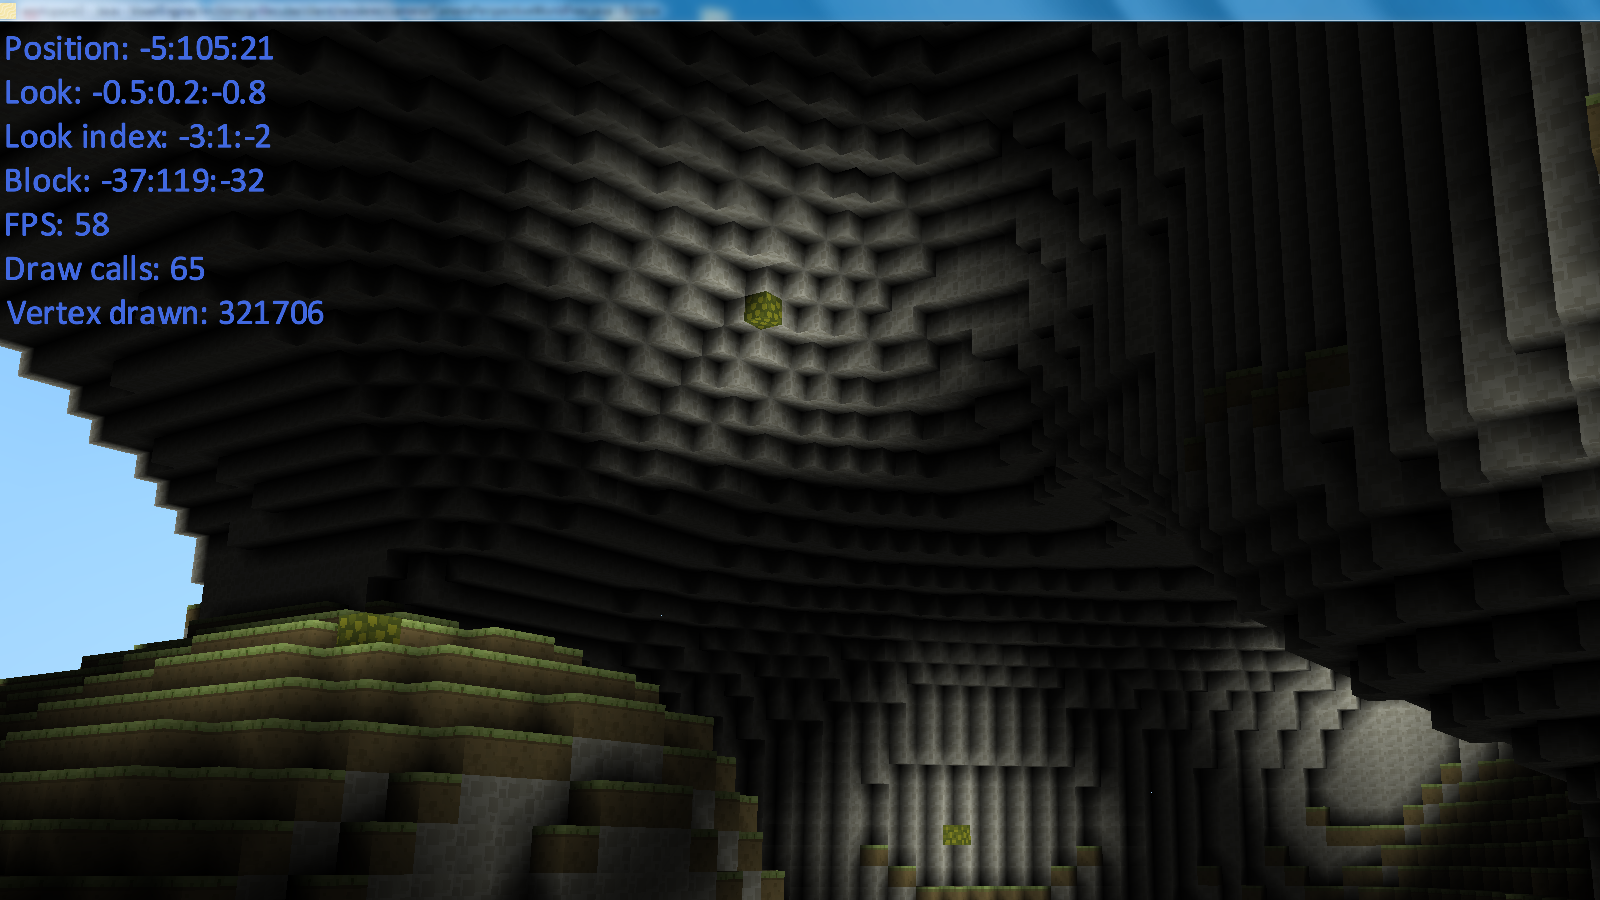
\includegraphics[width=0.6\textwidth,height=0.6\textheight,keepaspectratio]{./assets/title.png}
		\end{center}
		\caption{\textit{Illustration of the final result}}
		\label{Title illustration}
	\end{figure}
	\newpage

	% introduction
	\section{Introduction}
	\newpage

	% body
	\section{Materials and methods}
		\subsection{sub section 1}
			\subsubsection{subsub section a}
			\subsubsection{subsub section b}
		\subsection{sub section 2}
	\newpage
	
	% general conclusion, performances, what can be improved ...
	\section{General conclusion}
	\newpage
	
	% bibliography
	\nocite{*}
	\bibliographystyle{amsplain}
	\bibliography{bibliografie}

\end{document}